\documentclass[main.tex]{subfiles}
\begin{document}

Python 在 MacOS 和 Unix/Linux 操作系统是默认安装好的,
但版本一般是 \texttt{2.x},
且没有图形用户界面\index{图形用户界面, Graphic User Interface},
只适合在终端\index{终端, Terminal}命令行上进行交互运行或脚本运行。
微软视窗没有默认安装 Python。

本书采用 Python \texttt{3.x}。虽然可访问 \texttt{https://www.python.org/downloads/}安装 IDLE (Integrated Development and Learning Environment, 集成开发学习环境)\index{IDLE, 集成开发学习环境}\index{IDLE, 集成开发学习环境},但是这个安装可省去.这个 IDLE 是终端命令行式的,无图形用户界面.
而本书将在有图形用户界面的 IDE (Integrated Development Environment, 集成开发环境)\index{IDE, 集成开发环境} 里操作。

Python 有好几种免费的,且功能卓越的 IDE 软件,其中Spyder 和 Jupyter都包括在内Anaconda。Spyder提供一个优秀的开发平台和用户界面,进行 Python 的代码编辑、交互运行和图形绘制。Jupyter 也提供这样的开发平台,但它以互联网浏览器为用户界面,背后由一个本地网络服务器引擎在支持。其它很受欢迎并且为软件开发人员广泛使用的免费 IDE 有 Microsoft Visual Studio Code (https://code.visualstudio.com) 和 IntelliJ (Community 版本) (https://www.jetbrains.com).
这两种 IDE 支持除了 Python 以外的其它语言,如 Java,JavaScript,Node.js 和 C++ 等,但 Python 以及它的一些常用包和库需要另行安装和配置. Jetbrain 开发的 Intellij 和 Pycharm 都非常好. 但Intellij Ultimate 版和 PyCharm Professional 版都需要付费购买许可证, 而免费的 Intellij Community 版和 PyCharm Community 版不支持本书要使用的一些 Python 库. 本书主要使用Spyder,为开拓眼见我们也使用 Jupyter.


若只安装 Spyder,可访问
\texttt{https://www.spyder-ide.org} 。

若只安装 Jupyter,可访问
\texttt{https://www.Jupyter.org} 。

我们建议安装 Anaconda Navigator,以便可同时使用Spyder 和 Jupyter及其它。 Anaconda的网址是:

\,\,\,\,\texttt{https://www.anaconda.com} 。

\noindent 需要注意的是,Anaconda个人版本(Individual Edition)是免费的,而其它版本则不是。个人版本从

\,\,\,\,\texttt{https://www.anaconda.com/products/individual} 。

\noindent 下载安装。
安装好后,打开 Anaconda Navigator 所见如图 \ref{fig:2.1.1}。

\begin{figure}[h]
	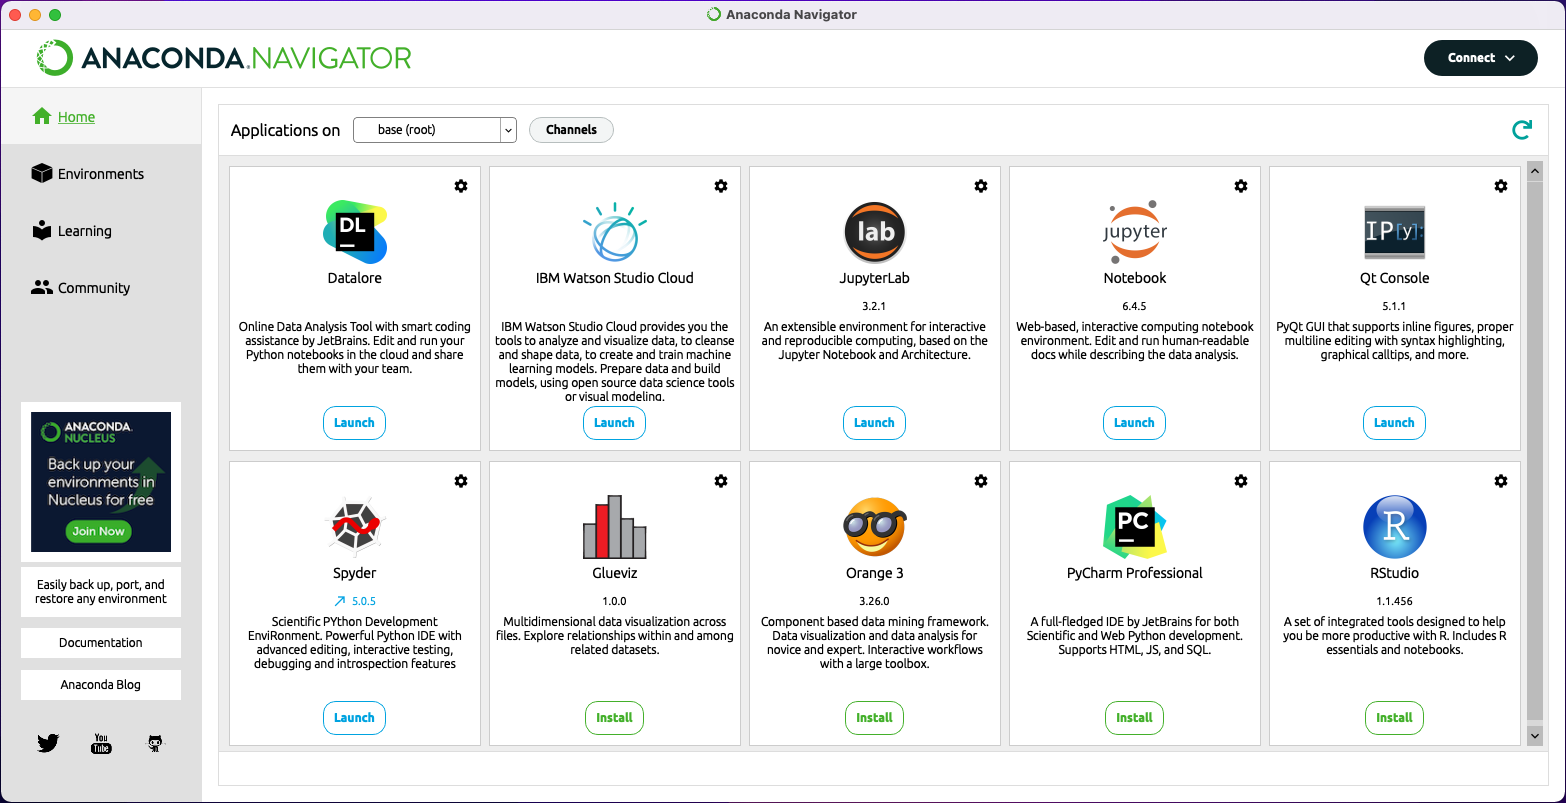
\includegraphics[width=1.0\textwidth]{png/anaconda_navig.png}
	\caption{Anaconda Navigator}\label{fig:2.1.1}
\end{figure}


conda install -c conda-forge jieba 

conda install -c conda-forge wordcloud
\end{document} 
